
\textbf{\textup{\huge {\bf Implementation: } \\[0.20in] }}

\normalsize { Each day an optimised path will be made by the system with respect to which all household have waste inside their dustbin(this info is taken via the dustbins internal system or the household user can manually override and prompt for a pick up) and the path is given for each collection vehicle to pick up waste and a notification is sent to each household to ask if they could give the waste at the specific time of the collections vehicles arrival, they could check the live location of the collection vehicle via the app and give their response. The path will be optimised again with respect to each household’s response. If the household didn’t or couldn’t give waste even after responding they could they will be fined.}\\[0.1in] 
\normalsize { 	When the collection vehicle comes near a specific household they could slide the dustbin out of a dock which houses the sensing and Wi-Fi system and give the dustbin to the collection worker, the worker would give a clean dustbin which was taken from the collection vehicle and take the full dustbin to replace it in the vehicle. The new clean dustbin can be slid back into the dock and the dock will read the RF ID chip which is every bin is equipped with and register the serial number of the bin, current date and the household where it has been placed into the systems server via home Wi-Fi. 
	. }\\[0.1in]
\normalsize {After the collection vehicle has done collecting it will go to the waste treatment plant and clear each of the bins if one of the bins are found to have mixed waste the source of the waste is found by tracking its serial number of the RF ID via the server’s database and that household would be fined. After all the dustbins are cleared, they are cleaned by pressurised water and circulated back. As each dock will register each time the dustbin is changed, we could count the number of days a specific house used the collection service and bill them accordingly so and each house hold could pay through our system and the collection workers will get the money via our system (like uber).}\\[0.01in]
\normalsize {The main way we will get the money for our services that is the two apps, the management system and the dustbins are by taking a fraction of the monthly profit of the collection workers and the interest of the caution deposit taken for each dustbin. The dustbin and the dock together is estimated to cost around 1200Rs per household and we will take a caution deposit of 600Rs from the households and give install it in their house, and 10 percentage of the monthly profit (excluding the fines collected from household for malpractice) of the collection workers will be taken by us. Although the dustbins are manufactured by us and given out for free of cost like a net router provided by a ISP but will still be owned by us. As for the cleaning of the dustbins must be done by the collection workers we will provide them the equipment for seemingly free of cost.
}\\[0.1in]

	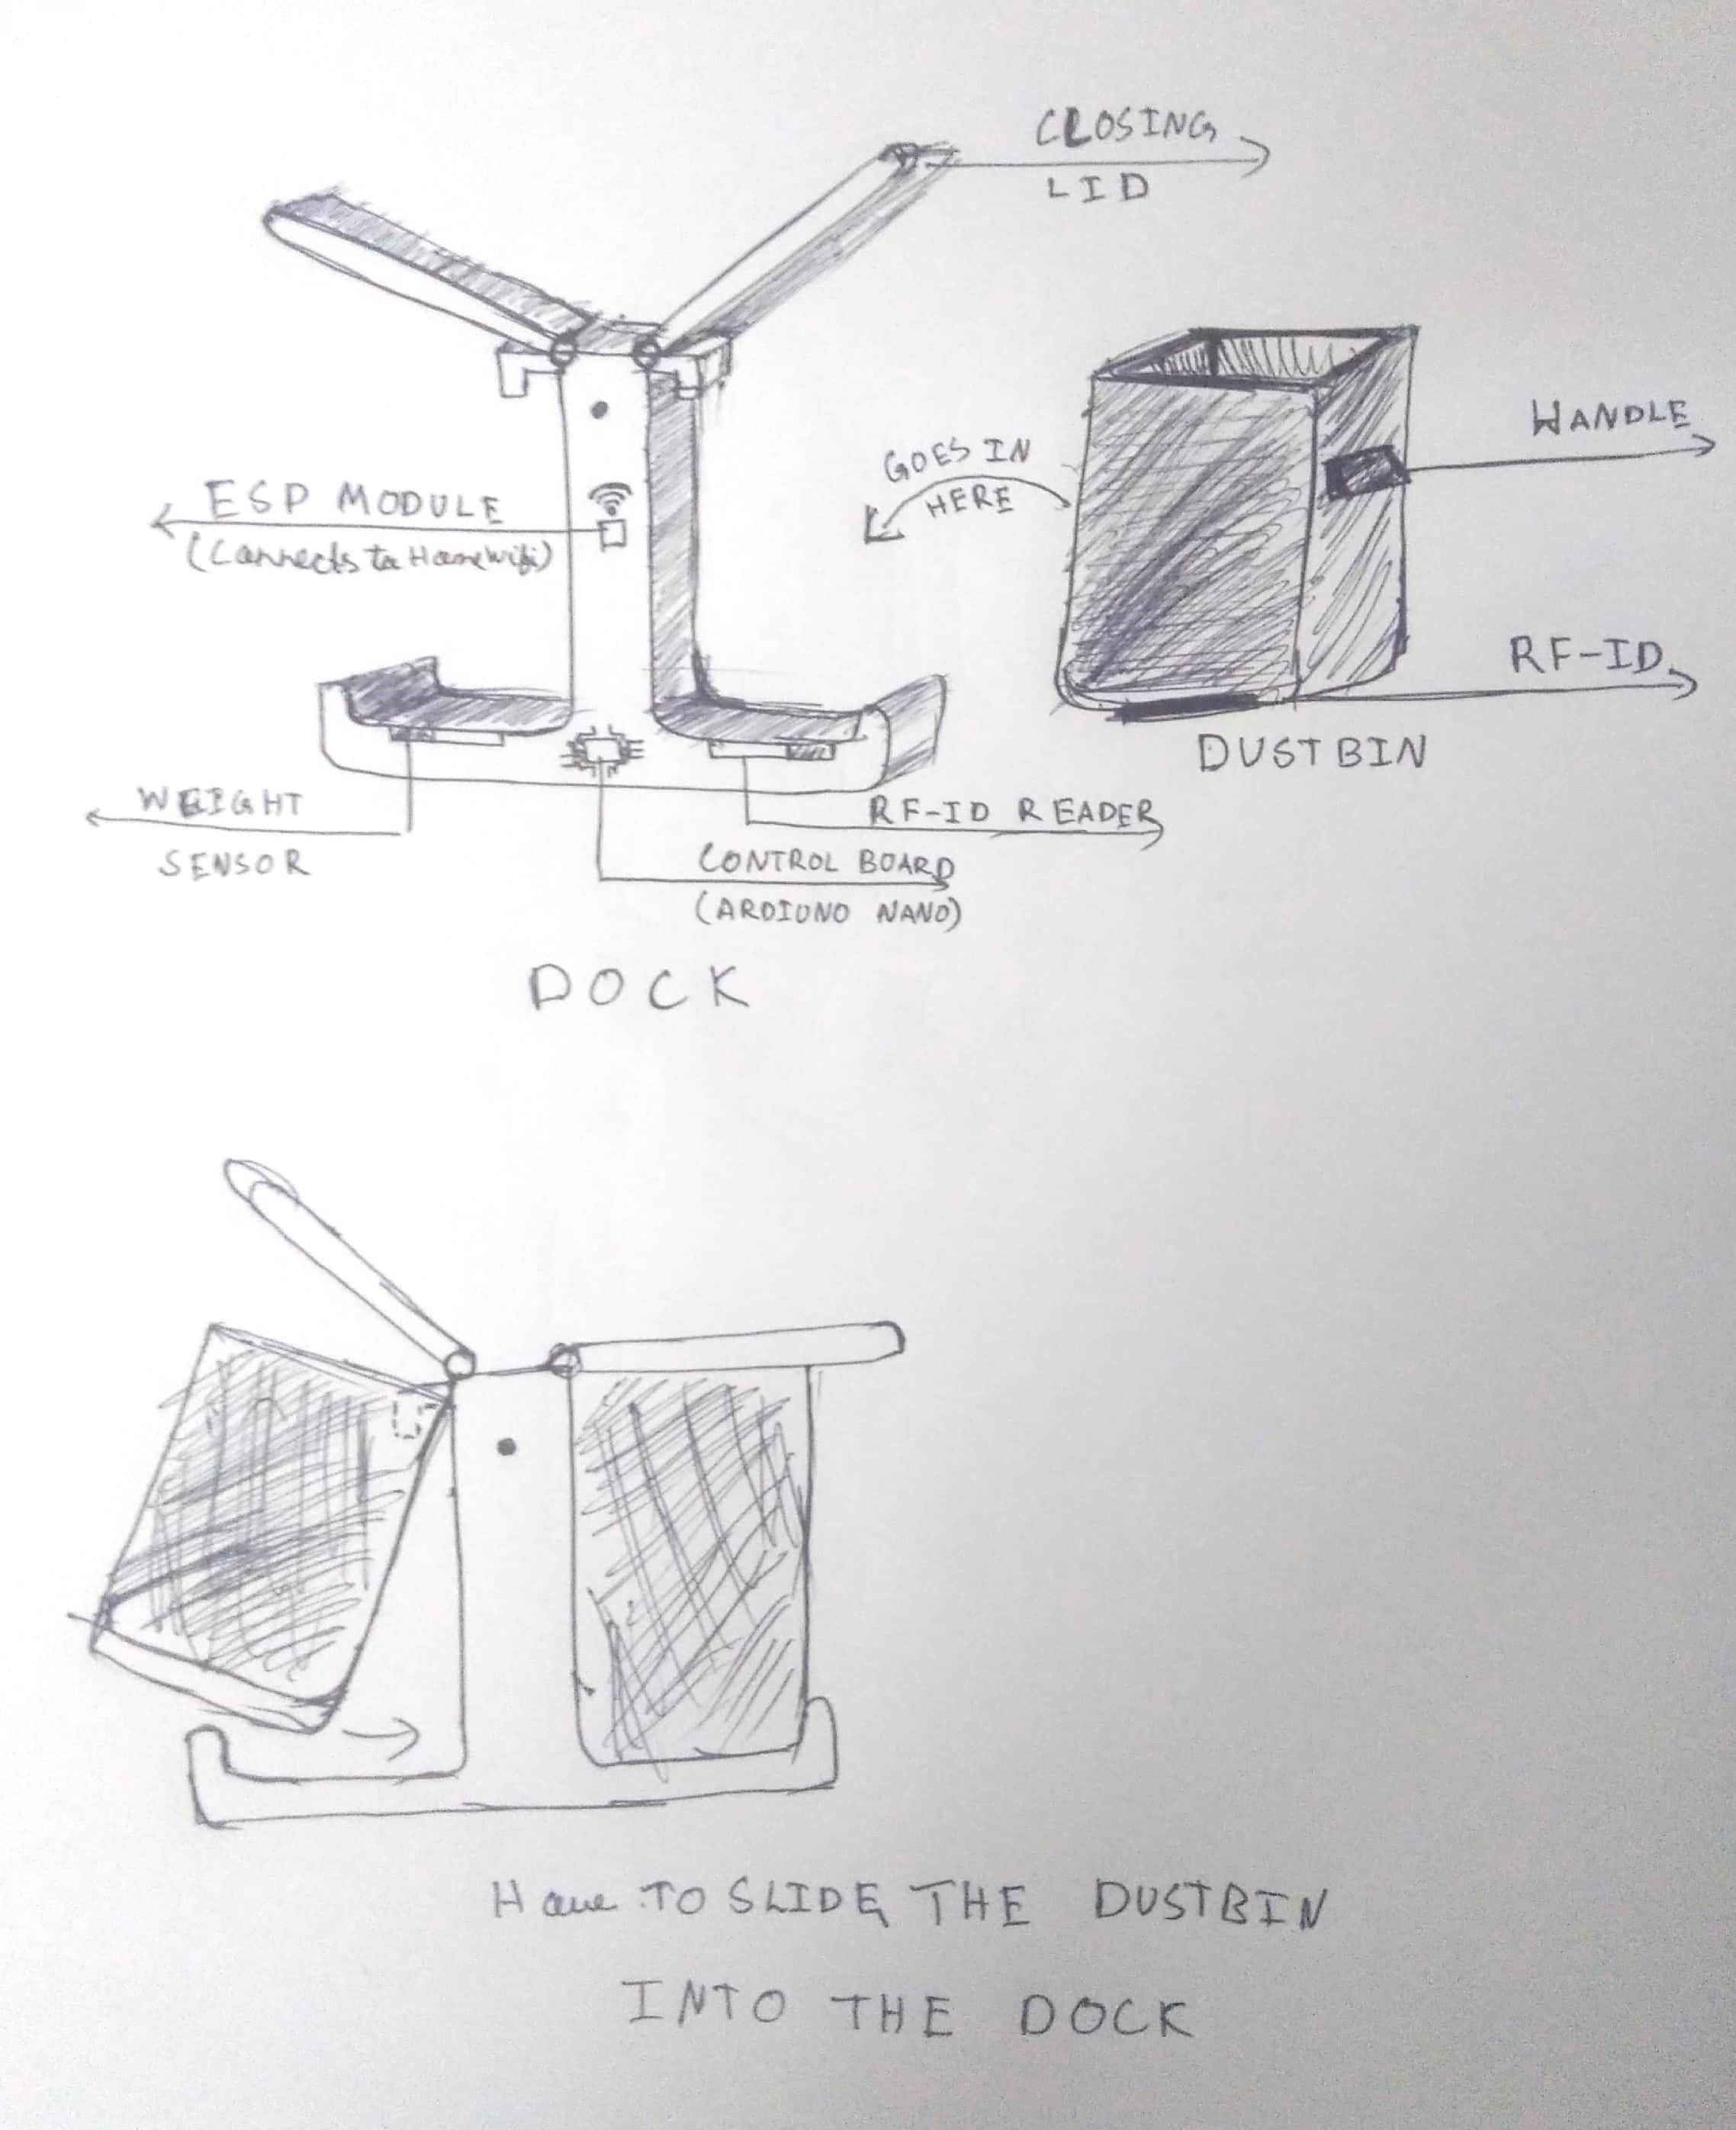
\includegraphics[width=\linewidth]{pic.jpg}
	
\newpage
